\documentclass{beamer}
\usetheme{Madrid} % 简洁清晰的Beamer主题
\usecolortheme{whale} % 沉稳配色,适配学术场景
\usepackage{ctex} % 中文支持
\usepackage{amsmath,amssymb,graphicx} % 公式与图形支持
\usepackage{hyperref} % 超链接

% 字体配置
\setCJKmainfont{SimSun} % 中文正文字体(宋体)
\setCJKsansfont{Microsoft YaHei} % 中文标题字体(微软雅黑)

% 课件基本信息
\title{现代控制理论研讨}
\subtitle{自适应控制的核心方法:Barbalat's lemma, PE 与其他}
\author{刘成}
\institute{中山大学 航空航天学院}
\date{\today}

\begin{document}




% ---------------------- 第1页:封面 ----------------------
\begin{frame}
  \titlepage
  \note{1分钟:封面页快速带过,明确课件主题是“参数估计”与“充分丰富信号”}
\end{frame}

\begin{frame}
  \frametitle{本ppt主要涉及}
  \begin{enumerate}
    \item 未知参数自适应 \footnote{\url{https://zhuanlan.zhihu.com/p/9450457498}}
    \item 未知控制方向自适应 \footnote{\url{https://zhuanlan.zhihu.com/p/9910889013}}
    \item 系统参数估计
    \item PE条件与barbalat 定理 
  \end{enumerate}
\end{frame}

% ---------------------- 第2页:目录 ----------------------
\begin{frame}{目录}
  \tableofcontents[sectionstyle=show/shaded, subsectionstyle=show/show/shaded]
  \note{1分钟:梳理课件逻辑,让听众明确核心模块}
\end{frame}


\section{Barbalat 引理}

\begin{frame}
  \frametitle{Barbalat 引理}
  \framesubtitle{函数及其导数的渐进性质}
  $\dot{f}\to 0 $
  $\nRightarrow$
  $f$ 收敛

  函数的倒数趋于零$\dot{f}\to 0 $并不等价于函数收敛$\exists C\in\mathbb{R},\lim_{t\to\infty}f(t)=C$.

  \begin{block}{example}
    \begin{enumerate}
      \item 有界函数:$f_1(t)=\sin(\ln t)$,$\dot{f}_1(t)=\frac{\cos(\ln t)}{t}$
      \item 无界函数:$f_2(t)=\sqrt{t} \sin(\ln t)$,$\dot{f}_2(t)=\frac{\sin(\ln t)}{2 \sqrt{t}}+ \frac{\cos (\ln t)}{\sqrt{t}}$
    \end{enumerate}

    这两个函数的导数都趋于零,但是函数不收敛.

    \begin{figure}
      \centering
      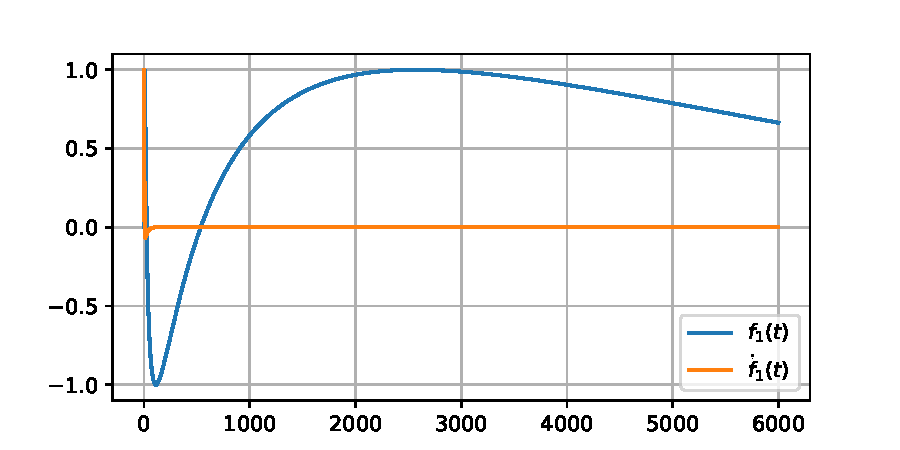
\includegraphics[height=2.8cm]{figure/sinlnt.pdf}
      \quad
      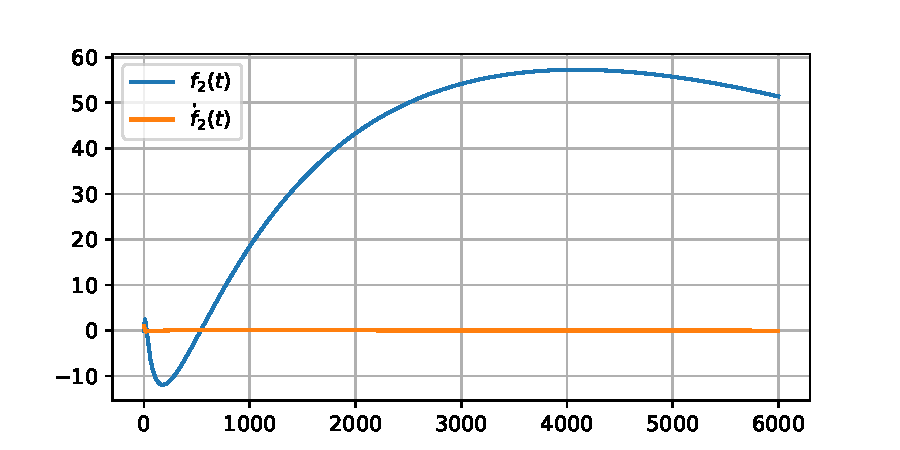
\includegraphics[height=2.8cm]{figure/sqrttsinlnt.pdf}
    \end{figure}
  \end{block}
\end{frame}

\begin{frame}
  \frametitle{Barbalat 引理}
  \framesubtitle{函数及其导数的渐进性质}

  $f$ 收敛
  $\nRightarrow$
  $\dot{f}\to 0 $

  函数收敛并不意味着函数倒数趋于零$\dot{f}\to 0$.

  \begin{block}{Tip: 与Lyapunov的联系}
    这个现象说明:
    如果一个函数$f$有下界并且为非增函数$\dot{f}\leq 0$,
    那么这个函数收敛到一个极限。
    \textbf{但是这个函数的导数不一定收敛到零}
  \end{block}

  \begin{block}{Example 1}
    另一个例子是周期脉冲信号:

    \begin{figure}
      \centering
      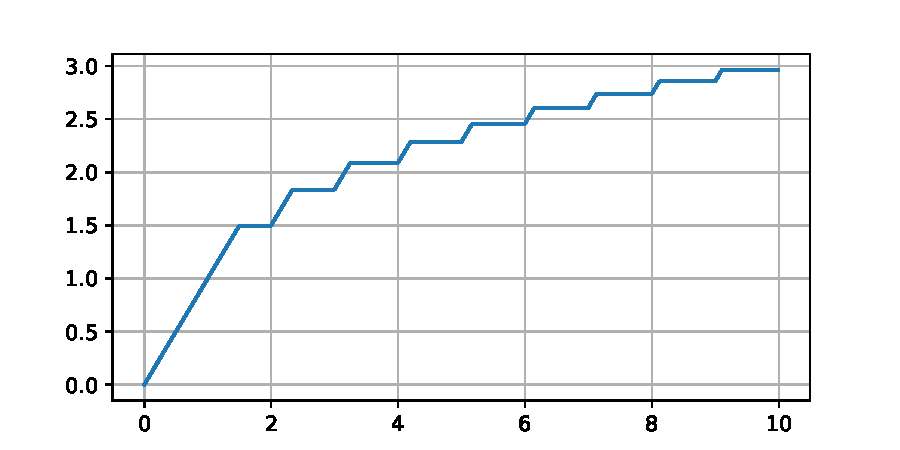
\includegraphics[height=2.6cm]{figure/barbalat_f4.pdf}
      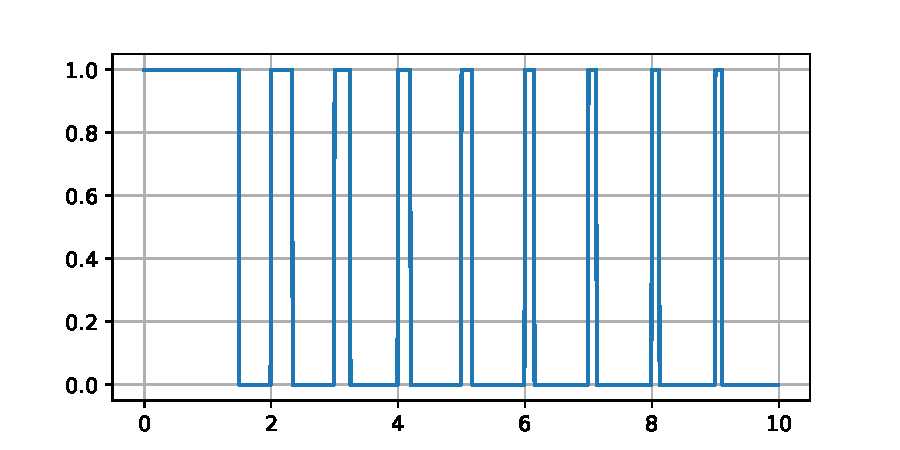
\includegraphics[height=2.6cm]{figure/barbalat_f4d.pdf}
    \end{figure}
  \end{block}
\end{frame}


\begin{frame}
  \begin{block}{Example 2}
    $f(t)=e^{-t}\sin (e^{2t})$收敛到零,但是其导数
    \[
      \dot{f}=-e^{-t}\sin(e^{2t}) + 2 e^{t} \cos(e^{2t})
    \]
    是一个有界函数。

    \begin{figure}
      \centering
      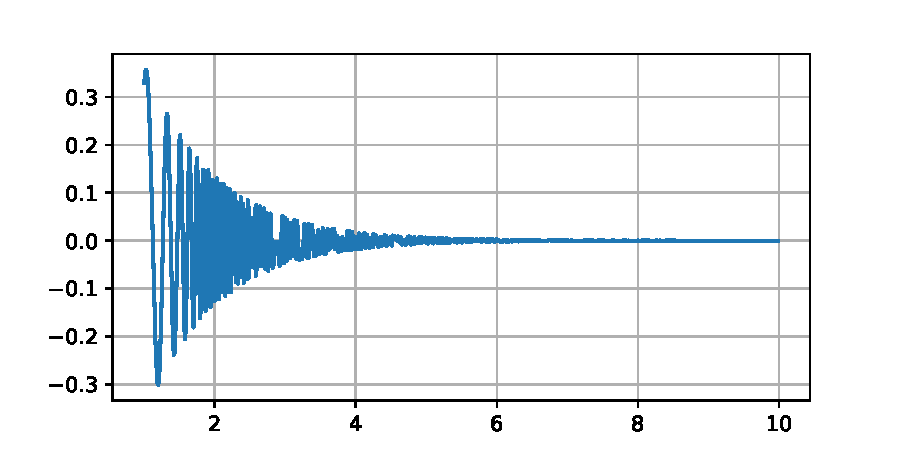
\includegraphics[height=2.6cm]{figure/barbalat_f3.pdf}
      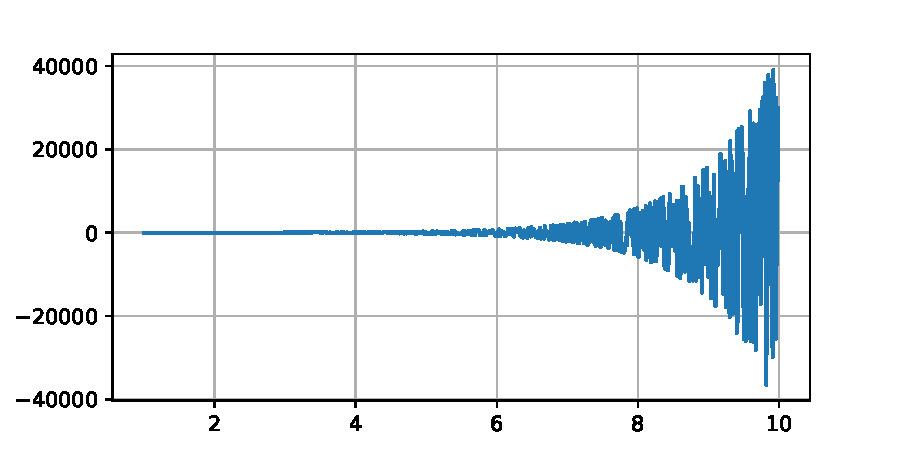
\includegraphics[height=2.6cm]{figure/barbalat_f3d.pdf}
    \end{figure}
  \end{block}
\end{frame}

\begin{frame}
  \frametitle{Barbalat‘s 引理的基本形式}

  \begin{lemma}
  设 $x:[0, \infty) \to \mathbb{R}$ 为一阶连续可导,且当 $t \to \infty$ 时有极限,则如果 $\dot{x}(t), t \in [0, \infty)$ 一致连续,那么 $\lim\limits_{t \to \infty} \dot{x}(t) = 0$。
  \end{lemma} 

  如果 $\ddot{x}(t)$ 存在且有界,那么引理1中 $\dot{x}(t)$ 的一致连续性条件可用 $\ddot{x}(t)$ 的有界性来替代,从而得到如下形式的引理。

  \begin{lemma}
  设 $x:[0, \infty) \to \mathbb{R}$ 一阶连续可导,且当 $t \to \infty$ 时有极限,则如果 $\ddot{x}(t), t \in [0, \infty)$ 存在且有界,那么 $\lim\limits_{t \to \infty} \dot{x}(t) = 0$。
  \end{lemma}

  如下推论是显而易见的。

  \begin{corollary}
    若 $x: [0, \infty) \to \mathbb{R}$ 一致连续,并且 $\lim\limits_{t \to \infty} \int_{0}^{t} x(\tau) \mathrm{d}\tau$ 存在且有界,那么 $\lim\limits_{t \to \infty} x(t) = 0$。
  \end{corollary}
\end{frame}

\begin{frame}
  \frametitle{在Lyapunov分析中的应用}  
  \begin{theorem}
    如果一个标量函数$V(t,x)$ 满足如下条件:
    \begin{enumerate}
      \item $V(t,x)$ 有下界;
      \item $\dot{V}(t,x)$ 是半负定;
      \item $\dot{V}(t,x)$ 关于时间是一致连续的
    \end{enumerate}
    那么 有$\lim_{t\to\infty} \dot{V}(t,x)=0$
  \end{theorem} 
\end{frame}

\end{document}